\chapter{Evaluation}
\label{ch:evaluation}

As a part of our work we prepared and performed a series of experiments with eZ430.
This chapter describes the motivation, methodology and results of those tests.  

\section{Power usage}

\subsection{Official specification}
Texas Instruments provides a specification of the eZ430 battery life (see Table \ref{tab:power-specification}).
It contains detailed data about the power usage of sensors and the pre-built eZ430 applications: BlueRobin and SimpliciTI.
Both of the applications are controlled from a PC using the Chronos Control Center (Figure \ref{fig:chronos_control_center}).

\begin{table}[h]
  \centering
    \begin{tabular}{|l|r|r|}
        \hline
        \textbf{Mode} & \textbf{Average Current} & \textbf{Battery Life} \\ \hline
        Shelf mode (LPM4) & 2.7 $\mu A$ & 92.6 months \\ \hline
        Welcome screen on the LCD (LPM3) & 8.9 $\mu A$ & 28.0 months \\ \hline
        Time/Date on the LCD & 9.0 $\mu A$ & 27.7 months \\ \hline
        Continuous temperature measurement & 10.0 $\mu A$ & 25.0 months \\ \hline
        Continuous altitude measurement & 18.0 $\mu A$ & 13.8 months \\ \hline
        Continuous acceleration measurement & 166.0 $\mu A$ & 1.5 months \\ \hline
        Continuous BlueRobin RX & 40.0 $\mu A$ & 6.2 months \\ \hline
        Continuous SimpliciTI PPT (no button pressed) & 10.0 $\mu A$ & 25.0 months \\ \hline
        Continuous SimpliciTI SYNC & 0.9 $m A$ & 8 days \\ \hline
        Continuous SimpliciTI ACC & 3.7 $m A$ & 2 days \\ \hline
        1h/day BlueRobin RX & 10.3 $\mu A$ & 24.2 months \\ \hline
        1h/day SimpliciTI PPT (no button pressed) & 9.1 $\mu A$ & 25.4 months \\ \hline
        1h/day SimpliciTI SYNC & 46.1 $\mu A$ & 5.4 months \\ \hline
        1h/day SimpliciTI ACC & 169.9 $\mu A$ & 1.4 months \\ \hline
    \end{tabular}
  \caption{eZ430 Chronos estimated battery life (from Texas Instrument User's Guide \cite{eZ430Chronos})}
  \label{tab:power-specification}
\end{table}

\begin{figure}[h]
  \centering
  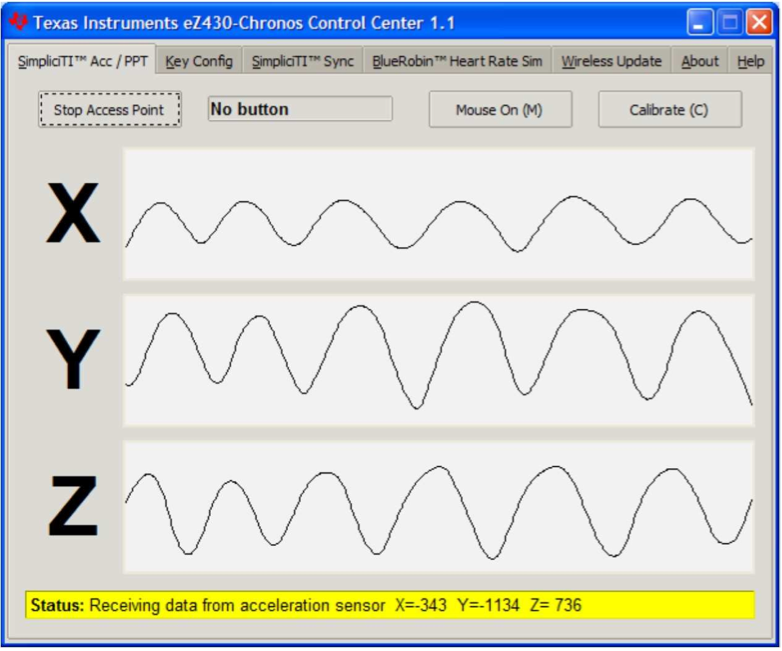
\includegraphics[width=0.6\textwidth]{img/chronos_app_control_center.png}
  \caption{Chronos Control Center PC Software (Courtesy of Texas
  Instruments)}
  \label{fig:chronos_control_center}
\end{figure}


BlueRobin\footnote{BlueRobin is a trademark of BM innovations GmbH} collects data from other ultra-low power sensors.
It supports retrieving heart beats from wireless belt.
In addition to that, it uses on-board eZ430 accelerometer to estimate speed and distance of person whose wear it.
Periodically, it transfers all those metrics through radio to a PC.
The application seems to be a proof of concept of watch for runners, similar to Adidas miCoach. 
It uses very little power, just a quarter of those required by using continously accelerometer alone.
However, it is impractical, because it requires user to be within radio range of a PC.

SimpliciTI\footnote{SimpliciTi is a trademark of Texas Instrument} is a versatile tool.
It consists of several modes.
PowerPoint Control mode (PPT) allows to map eZ430 buttons to PC keys.
That way a user can control a presentation, a music player, etc.
Acceleration data mode (ACC) enables transmitting eZ430 acceleration data to a PC through the radio.
It is also possible to control a PC mouse using the accelerometer data.
Synchronization mode (SYNC) allows for calibration of the device sensors and setting the time on eZ430 from a PC.
In addition to that, SimpliciTI provides standard watch functionality, such as clock, timer, alarm, etc. 

However, Important details, such as duty cycle and radio transfer rate are not specified for both applications.
Moreover, there are no data about the most power intensive operations: receiving and sending radio packets.
Such operations consume orders of magnitude more energy, than those listed in Table \ref{tab:power-specification}.
Therefore, having detailed measurements is required to do accurate battery life estimations.

\subsection{Low-power listening}
Overall, listening is usually the most power-expensive operation, largerly, because the majority of applications spend much more time listening than sending the data.
In order to reduce the listening time, TinyOS supports low-power listening (LPL).
However, sending data to node using LPL uses more energy.

In LPL, a listener node, periodically (e.g. every 200 ms) performs clear channel assasment (CCA).
If the check detects communication, it veryfies whether it is a sender's preamble.
If it is so, it starts regular radio listening, until the end of communication.

On the other hand, sender has to prelude its packet with a preamble of length at least equal to interval between listener's CCA checks.
A preamble is pre-defined by protocol and consist of repeated signal pattern.
That way, the listener node will always perform periodical check during sender's preamble and could easily identify it.
Having that, after the preamble, both nodes have turned on radio and the sender could transmit packet to the listener.

The example communication is showed in Figure \ref{fig:low_power_listening}.
In addition to that, nodes could continue communication, after the first sender's packet.
However, if there are no transmissions, both nodes return to the original state.
This allows to minimize overhead caused by preamble.

\begin{figure}[h]
  \centering
  \includegraphics[width=0.6\textwidth]{diagrams/low_power_listening.eps}
  \caption{Timeline of communication with low-power listening}
  \label{fig:low_power_listening}
\end{figure}

\subsection{Test setup and methodology}

\begin{figure}[h]
  \centering
  \includegraphics[width=0.4\textwidth]{diagrams/power.eps}
  \caption{Power measurement setup}
  \label{fig:power}
\end{figure}

% schema
Even though, we did not have a device that could measure electric current directly over time, we were able to calculate the current indirectly using Ohm's Law: 

$$
U = I \cdot R
$$

The law states that the potential difference on a resistor (U) is equal to the current (I) flowing through the resistor divided by its resistance (R).
In our setup, we knew the resistance of the resistor in Ohm and could measure the voltage drop using an oscilloscope (Figure \ref{fig:power}).
Therefore, we are able to calculate the electric current.
However, Ohm's law describes an ideal resistor.
In contrast, our testing setup does not fulfil all of the assumptions.
In particular, we a got a 20 $mV$ baseline difference in potential, which is subtracted from the final measurements.

The oscilloscope used was Owon PDS 5022S (see Figure \ref{fig:owon}).
It is capable of plotting voltage difference with a $ 0.1 ms$ accuracy.

\begin{figure}[h]
  \centering
  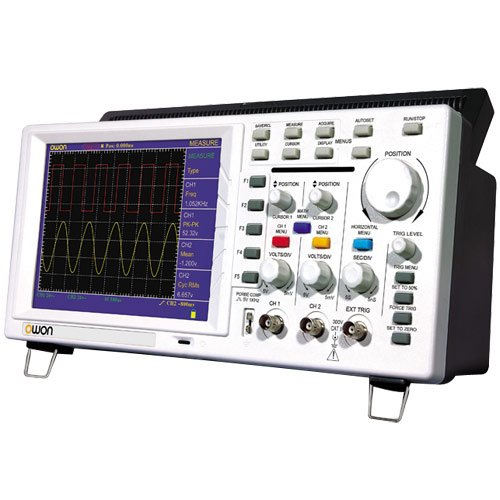
\includegraphics[width=0.4\textwidth]{img/owon_pds5022s.jpg}
  \caption{Owon PDS5022S oscilloscope (courtesy to the manufacturer)}
  \label{fig:owon}
\end{figure}

Instead of batteries, a 3 V direct current (DC) power adapter was used as the power source in order to provide a consistent voltage.

Having that setup we ran series of tests.
Each one begins with programming an eZ430 with a special purpose application, described in Table \ref{tab:power-apps}.
Every application ran for a few minutes, pausing the plot several times and recording the voltage difference.
A video was recorded for verification purposes.
As a final measure, we take the average of observations with a 1 $ mV $ accuracy.

For most of the tests the, the voltage drop was almost constant.
However, their are certain operations which could not be performed on eZ430 continuously.
In particular, sending series of radio packets is not possible without switching the radio to receiving mode between each transmission.
Therefore, the sending power consumption was measured only when actual packets were sent.

A similar issue appeared in low-power listening, where we measured the top power consumption of a receive check.


\begin{table}
  \centering
    \begin{tabular}{|l|l|}
        \hline
    \textbf{Application} & \textbf{Description} \\ \hline
    Null app & sleeps all the time \\ \hline
    LCDDriverTest App & uses LCD display intensively \\ \hline
    Loop & perform non-stop computations at 8 MHz \\ \hline
    TestAccelerator & Reads in a loop the acceleration reading, \\
    & unintentionally it is also maxing out CPU \\ \hline
    Radio listening & listen on radio (no difference whether it gets packets) \\ \hline
    Low-power listening & wakes every X $ ms $ to check if someone transmits on radio \\ \hline
    Sending at maximal power & sends packets with strongest signal - at +12 $ dB $ \\ \hline
    Sending at minimal power & sends packets with weakest signal - at -30 $ dB $ \\ \hline
    \end{tabular}
  \caption{Special purpose application used to measure power usage}
  \label{tab:power-apps}
\end{table}

\subsection{Results}

Our equipment was good enough to measure radio-related operations with a reasonable accuracy (see Table \ref{tab:power-usage}).
In contrast, the onboard sensors consume too little energy to be above the noise.

However, our results are complementary to the official specification.
Combing both data sources it is possible to estimate the energy budget of a real-world application.

For example, we might assume that our application will listen for $2 \%$i of the time, send for $ 0.1 \% $ and use accelerometer for $ 10 \% $.
Under these assumption, the estimated average power usage of the application will be:
\begin{equation}
0.1 \% \cdot 27 mA + 1 \% \cdot 10 mA + 10 \% \cdot 166 \mu A + 90 \% \cdot 8 \mu A = 0.1508 mA   
  \label{eqn:power_example}
\end{equation}
Which gives a battery life of:
$$
\frac{190}{0.1508} \approx 1260 h \approx 52 days
$$
(assuming 190 mAh CR2032)



\begin{table}[h]
  \centering
    \begin{tabular}{|l|r|r|r|}
        \hline
              & \textbf{I (estimated)} & \textbf{I (measured)}          & \textbf{Voltage drop on resistor}  \\ \hline
Baseline & - & - & 20 $ mV $ \\ \hline
Null app    & - & 3 $ mA $          & 20 $ mV $  \\ \hline
LCDDriverTest app    & - & 3 $ mA $ & 20 $ mV $  \\ \hline
Loop    & 1 $ mA $ & 4 $ mA $          & 28 $ mV $  \\ \hline
TestAccelerator     & 1 $ mA $ & 4 $ mA $          & 28 $ mV $  \\ \hline
Radio listening     & 16 $ mA $ & 19 $ mA $   & 130 $ mV $  \\ \hline
Low-power listening     & 10 $ mA $ & 13 $ mA $              & 88 $ mV $  \\ \hline
Sending at maximal power     & 27 $ mA $ & 30 $ mA $              & 206 $ mV $  \\ \hline
Sending at minimal power      & 12 $ mA $ & 15 $ mA $            & 102 $ mV $  \\ \hline

    \end{tabular}
  \caption{eZ430 Chronos measured battery life}
  \label{tab:power-usage}
\end{table}

\subsection{Energy cost of low-power listening}

Listening and sending the data takes roughly the same amount of power as described in Table \ref{tab:power-usage}.
Also sending a preamble consumes the same amount of power as sending the data.
The only unknown is thus how much power a receive check costs.

A single check uses clear channel assessment, which could give a false positive, but uses less power than listening.
It takes 4 $ ms $ with the average 5 $ mA $ current during the whole check (see Figure \ref{fig:low_power_receive_check}).

\begin{figure}[h]
  \centering
  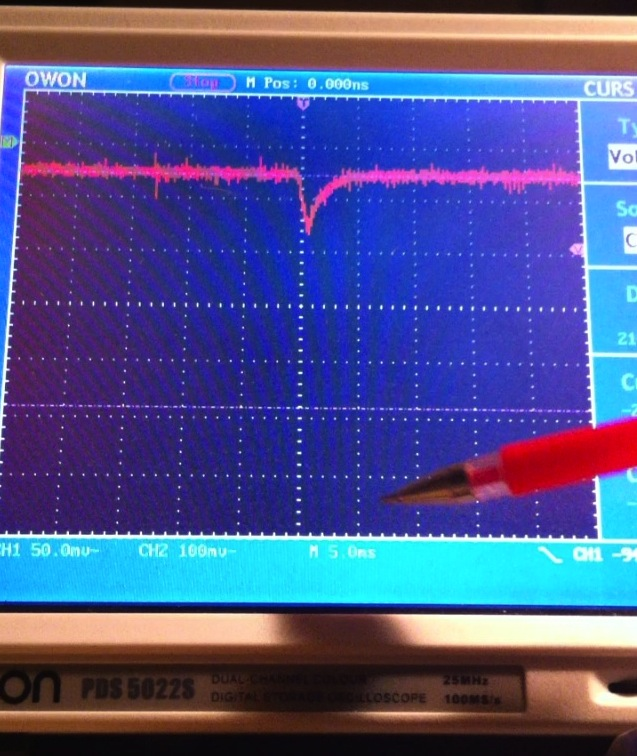
\includegraphics[width=0.6\textwidth]{img/low_power_receive_check.jpg}
  \caption{Inverted graph, low peak: $ 88 mV$, top line: 20 $ mV $}
  \label{fig:low_power_receive_check}
\end{figure}

For example, idly listening with LPL with a 250 $ ms $ sleep interval consumes:
$$
\frac{4 \cdot 4 ms \cdot 5 mA}{1000 ms} \approx 0.08 mA
$$
In addition to that, we need to calculate the power consumption of an actual transfer.
Let say we transfer take 50 $ ms $ every 30 $ s $, also we will be listening on average half of the preamble: $\frac{250 ms}{2} =  125 ms$.

So the listener uses:
$$
\frac{(125 ms + 50 ms) \cdot 16 mA}{30 \cdot 1000 ms}  + 0.08 mA \approx 0.09 mA + 0.08 mA = 0.17 mA
$$

While sender node uses:
$$
\frac{(250 + 50) ms \cdot 30 mA}{30 \cdot 1000 ms} \approx 0.3 mA
$$

\subsection{Other considerations}
In the real world, there are many other factor that affect the battery life.
For example, battery capacity depends on temperature and is usually lower than are specified by the manufacturer.
Because of that, real world applications have shorter battery lives than what estimations would suggest.


\section{Radio range}

Range is one of the most important parameters of a radio module.
However, there is no official specification of the eZ430 range.
The user documentation (\cite{eZ430Chronos}) gives only a vague description:
\begin{quote}
In free field distances of up to 100 m (328 ft) have been measured. The range in other conditions,
especially within buildings, is hard to predict.
\end{quote}

That kind of description is definitely not sufficient.
As an application developer, we are interested not only in the maximum range, but also in the transfer reliability.


\subsection{Methodology}

As part of the evaluation we did line-of-sight tests in a park.
We used two watches that could ``see'' each other, with no objects between them.
Radios were configured for the 868 MHz frequency with a 250 kbit transmission rate.
All watches were fully assembled and placed about 80 $ cm $ above the ground.
The power was supplied by previously unused CR2032 batteries, which were replaced in the middle of the tests to provide a more consistent environment.

The test consisted of sending 100 20-byte packets.
Between each packet, there was a 256 $ ms $ sleeping interval.
During the test s watch was rotated to simulate real hand movements.
After each test, the data was sent to a PC using radio printf and a GNode as a bridge.

It took a few iteration to produce results which were repeatable.
Tests inside of building, without line-of-sight, with used batteries or with fixed watch rotation result in inconsistent or hard to reproduce data.

All these tasks were performed using a ChronosConnectivityAssesment application.
The application provides a user interface using the LCD and buttons.
One of it its features is the ability to change the radio output power level.

For all tests we collected the following three metrics:
\begin{itemize}
  \item \textbf{reliability} --- packets received
  \item \textbf{average RSSI} --- the amount of received signal strength indication (RSSI), provided by hardware.
  \item \textbf{average LQI} --- Link quality indicator (LQI), a heuristic quality value provided by the radio chip.
\end{itemize}

Each test were performed with three different radio strength: +12 dB (maximal), 0 dB and -30 dB (minimal).

All distances are in meters, except the one denoted ``next''  which meant closest possible within a given radio strength.
Placing two watches closer than this distance disables radio communication completely.
``Next'' is about $20 cm$ for $+12 dB$ and close to $0 cm$ for $- 30 dB$.

% methodology

% Chronos connectivity

\subsection{Reliability results}

The results data show that radio got range of about $50$ meters.
Within short distance, there are very few packets lost\footnote{in our environment there are almost no collisions}.
However, There is a sharp drop in reliability after certain distance.
This is excepted, as free-space path loss is square proportional to the distance from the source.

Although, radio strength -30 dB may seems impractical, it is a good method to detect whether sender is close ($< 2m$) to the receiver.

Overall, radio chip in eZ430 is relaible and provide reasonable radio range.


\subsubsection{+12 dB}

\begin{figure}[H]
  \centering
  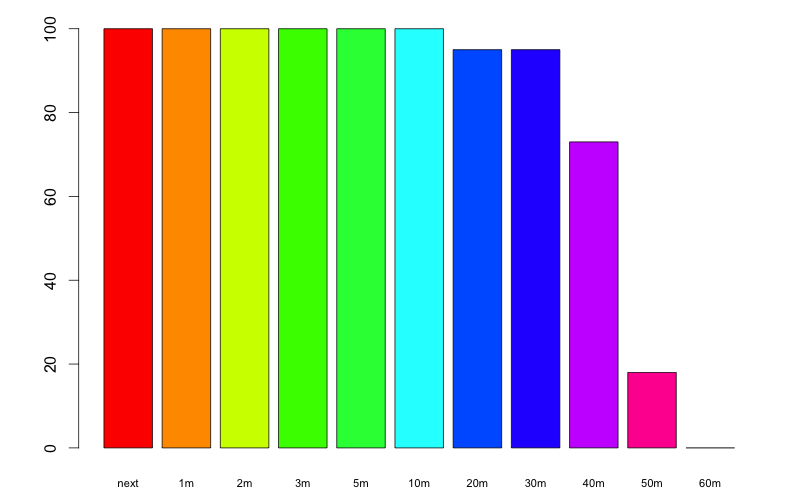
\includegraphics[width=0.9\textwidth]{img/tests/range/db_12.png}
\end{figure}


\subsubsection{0 dB}

\begin{figure}[H]
  \centering
  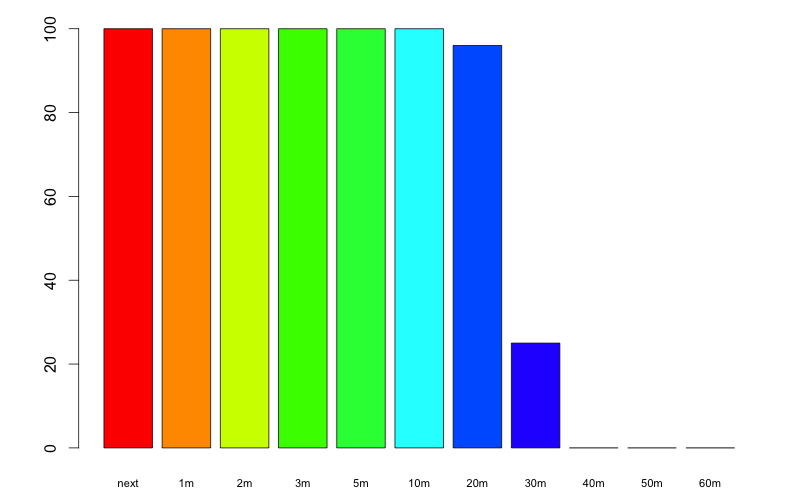
\includegraphics[width=0.9\textwidth]{img/tests/range/db_00.png}
\end{figure}

\subsubsection{-30 dB}

\begin{figure}[H]
  \centering
  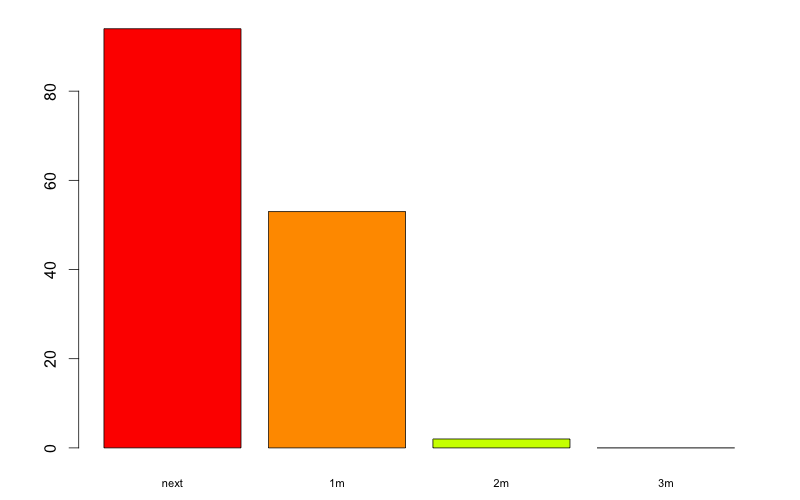
\includegraphics[width=0.9\textwidth]{img/tests/range/db_m30.png}
\end{figure}

\subsection{RSSI results}


The RSSI results are presented as box plots.
The thick line shows the median.
The box edges are on 1st and 3rd quartile.
The top and bottom lines are correspondingly the minimal and the maximal element.
Each point which is more than 1.5 times away than the height of the box is considered as an outlier and marked with a circle.

RSSI is usually used to determine the quality of radio communication.
It may be also utilized to estimate the distance between a sender and a listener.
Though, single measurement may be misleading, a median from series of transmissions is a good indicator.


\subsubsection{+12 dB}

\begin{figure}[H]
  \centering
  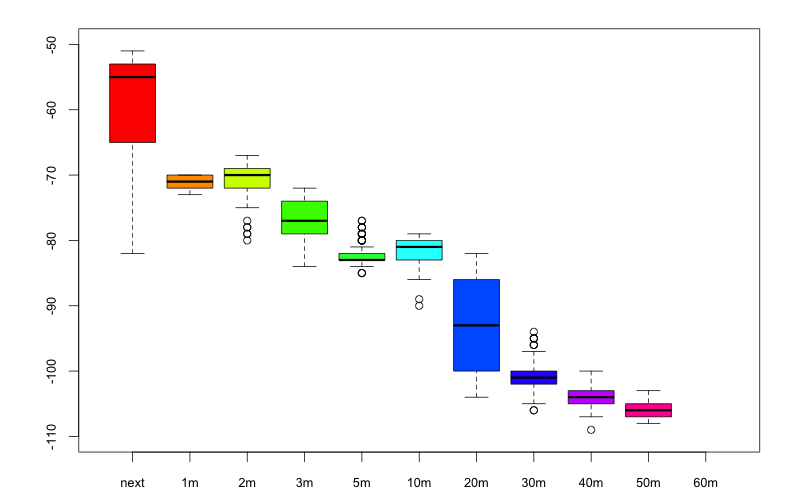
\includegraphics[width=0.9\textwidth]{img/tests/rssi/db_12.png}
\end{figure}


\subsubsection{0 dB}

\begin{figure}[H]
  \centering
  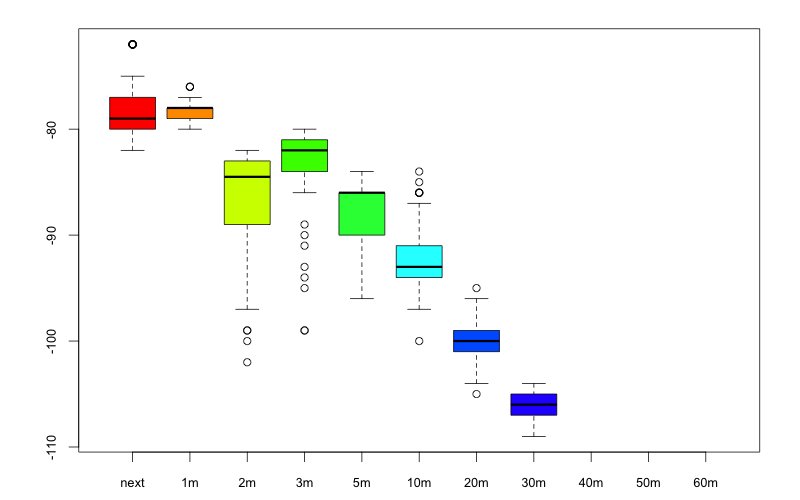
\includegraphics[width=0.9\textwidth]{img/tests/rssi/db_00.png}
\end{figure}

\subsubsection{-30 dB}

\begin{figure}[H]
  \centering
  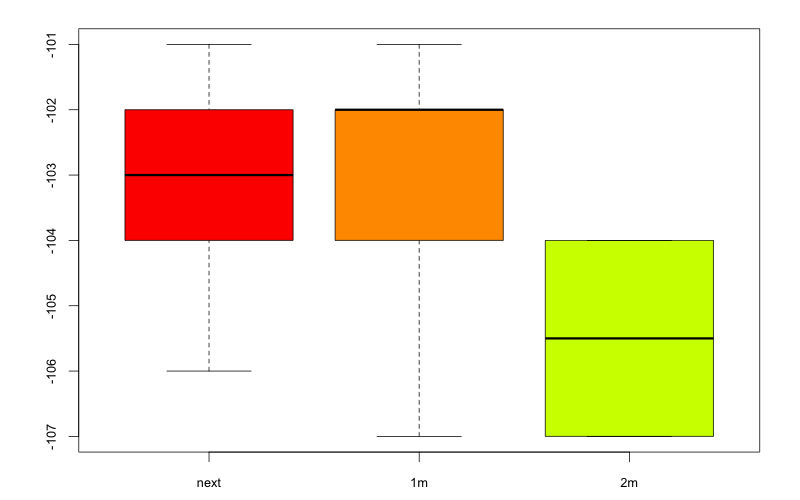
\includegraphics[width=0.9\textwidth]{img/tests/rssi/db_m30.png}
\end{figure}

\subsection{LQI results}
The LQI results have same form as the RSSI results.

LQI is an alternative metric to RSSI.
Even from a signal LQI data point gives a good prediction of packet loss.
However, it is a bad metric to estimate the distance and RSSI should be used for that purpose instead.


\subsubsection{+12 dB}

\begin{figure}[H]
  \centering
  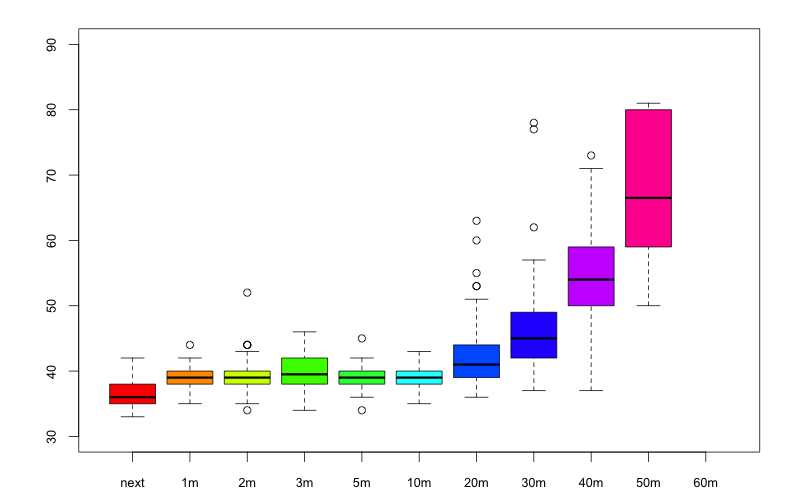
\includegraphics[width=0.9\textwidth]{img/tests/lqi/db_12.png}
\end{figure}


\subsubsection{0 dB}

\begin{figure}[H]
  \centering
  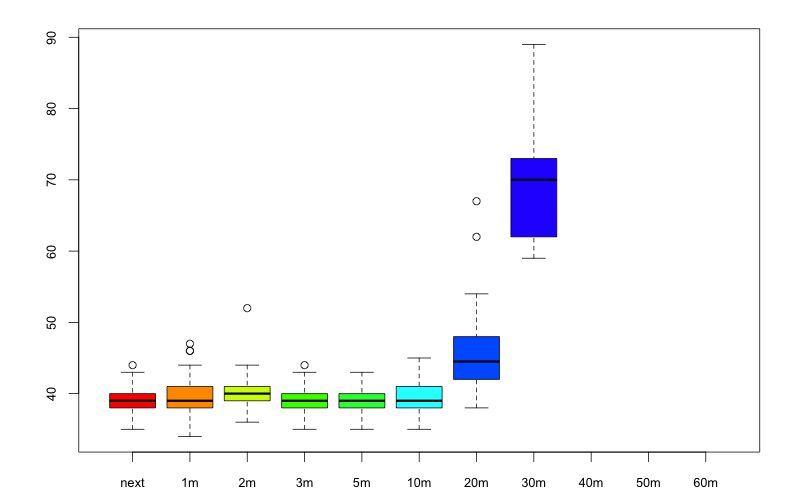
\includegraphics[width=0.9\textwidth]{img/tests/lqi/db_00.png}
\end{figure}

\subsubsection{-30 dB}

\begin{figure}[H]
  \centering
  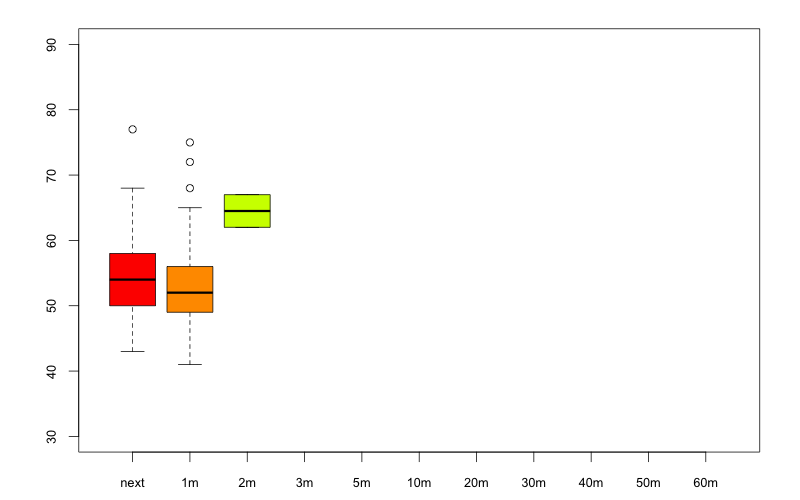
\includegraphics[width=0.9\textwidth]{img/tests/lqi/db_m30.png}
\end{figure}

% results

\section{Radio throughput}

% methodology
The theoretical throughput is 250 kbits.
However, the communication requires sending frame header and footer (11 and 3 bytes respectively) for each packet.
The packet maximal size is 64 bytes, so at most 50 bytes remains for payload.
In addition to that, the radio driver performs clean channel assessment before each transfer.
This reduces packet collisions, but reduce the bandwidth.
Moreover, in practical applications we also need to take into account time needed to copy memory block of packet payload.


% results
We performed series of experiments which measure the throughput, which we define as a rate of successful delivered total size of payload.
The watches were placed close to each other, MCU frequency was set to 8 MHz and radio baud rate to 250 kbits.
In this setup packet delivery failure was negligible.
As excepted, the measured bandwidth in Table \ref{tab:radio-throughput} is fraction ($\frac{250}{6.10 \cdot 8} \approx 5.1$) of theoretical throughput.

\begin{table}[h]
  \centering
    \begin{tabular}{|r|r|r|}
        \hline
        \textbf{Payload size in packet} & \textbf{Time required to send 1000 packets} & \textbf{Throughput} \\ \hline
        50 bytes& 8.2 s & 6.10 KBps \\ \hline
        30 bytes& 6.5 s & 4.46 KBps \\ \hline
        10 bytes& 5.1 s & 1.96 KBps \\ \hline
    \end{tabular}
  \caption{eZ430 Chronos radio throughput}
  \label{tab:radio-throughput}
\end{table}



\section{Sample application: Zordon}

Also as part of evaluation, we implemented sample application.
Each watch is associated with a name and has the radio in low-power listening mode.
A user select one of the names from the LCD menu, then he could send a beep request over radio.
If the watch receives beep request addressed to its name, it plays a sound using a built-in buzzer and displays the sender's name.

This application can be used to call friends who are in nearby rooms.
It is a useful example which shows the major TinyOS advantage: it allows to write application just by describing its logic without worrying about underlying hardware.



% Use case


% \Bump

% \ CTP
